\documentclass[border=1pt,tikz,varwidth=\maxdimen]{standalone}

\usetikzlibrary{positioning,calc,arrows.meta}

\begin{document}
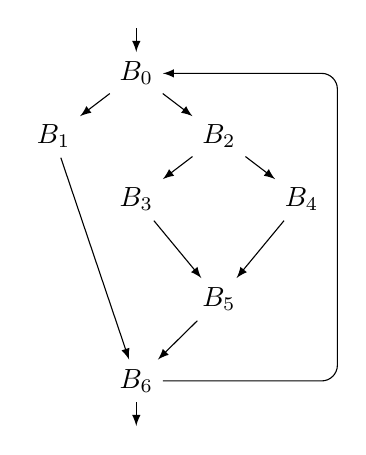
\begin{tikzpicture}[
  level distance = 8mm,
  sibling distance = 21mm,
  arrow/.style={edge from parent/.style={solid,draw,-latex}},
  empty/.style={edge from parent/.style={}},
  rounded-arrow/.style={-latex,rounded corners=2mm,>=Stealth[round]},
  ]
  \coordinate (start);
  \node [below=2ex of start] (B0) {\(B_{0}\)}
  child [arrow] {
    node (B1) {\(B_{1}\)}
    child [empty] {
      node {}
      child {
        node (empty5) {}
      }
    }
  }
  child [arrow] {
    node (B2) {\(B_{2}\)}
    child {
      node (B3) {\(B_{3}\)}
    }
    child {
      node (B4) {\(B_{4}\)}
      child {
        node [below=of $(B3)!0.5!(B4)$] (B5) {\(B_{5}\)}
        child {
          node [below=of $(B5)!0.5!(empty5)$] (B6) {\(B_{6}\)}
        }
      }
    }
  };
  \coordinate [below=2ex of B6] (end);

  \draw [-latex] (start) -- (B0);
  \draw [-latex] (B6)    -- (end);

  \coordinate [right=3ex of B6 -| B4] (temp);
  \draw [-latex] (B1) -- (B6);
  \draw [-latex] (B3) -- (B5);
  \draw [rounded-arrow] (B6) -- (temp) |- (B0);
\end{tikzpicture}
\end{document}
